\chapter{THEORETICAL BACKGROUND} \label{chapter:theoretical_backgroundpape}
    \section{Neural Networks (NNs)} \label{sec:nn}
    The human nervous system contains cells, called neurons. The neurons are connected to each another through axons and dendrites, the regions between which, are known as synapses(synaptic connections). In the presence of external stimuli, the strengths of synaptic connections are often differentiated, which is exactly how living organisms learn. 

      \begin{figure}[h]
        \centering
        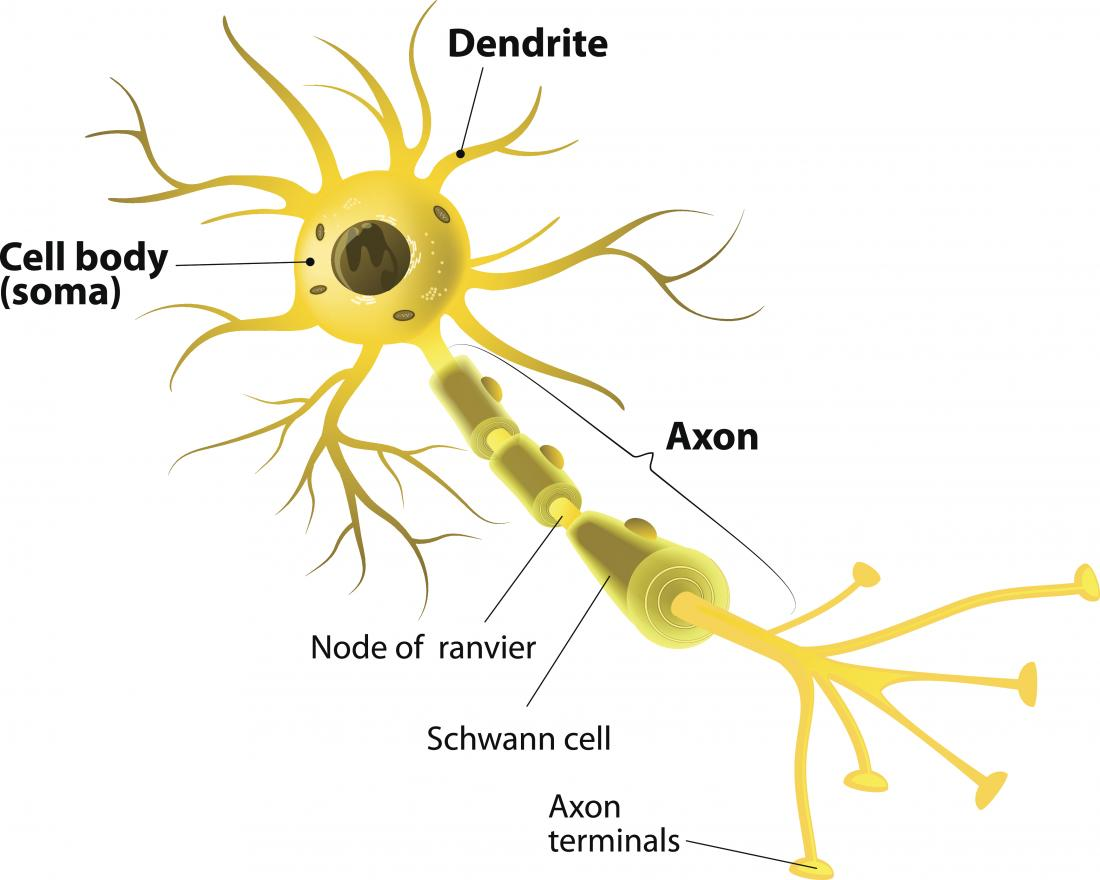
\includegraphics[width=0.65\textwidth]{media/neuron-diagram.jpg}
        \caption{Human Neuron}
        \label{fig:humanNeuron}
    \end{figure}

    
    Human neurons consist of three main parts: dendrites, the cell body and axons. Dendrites are thin filaments that carry information from other neurons to the soma of the neuron they are part of, so they are the input part of the cell. Soma (cell body) contains the neuron's nucleus and receives information through the dendrites. Axon is a long projection that transfers information from the soma to other cells in the system, so it is the output part of the cell. It normally ends with a number of synapses connected to the dendrites of other neurons.

    Artificial Neural Networks (ANNs) were made to mimic the biological mechanism explained above. They consist of units or nodes, referred to as neurons, which perform all the necessary computations. Those units are interconnected through weights, which have the same role as the strengths of synapses in the biological process. Each input to a neuron is scaled with a weight, which has impact on the function that this particular unit computes. An ANN computes a function of the inputs by propagating the computed values from the input nodes to the output node(s). The weights are parameters which undergo changes, in order for the learning process to take place. During that learning process, the network is being fed sets of training data containing examples of input-output pairs of the function to be learned, using the input representations to make predictions about the output labels. The training data provides the feedback needed to properly adjust the weights of the NN, a task that depends on how well the predicted output (e.g., probability of a C note -- Do) for a particular input, matches the output label in the training data. The goal of changing the weights is to optimise the computed function to predict more accurately in the next iterations. When a NN is trained with many different samples sharing the same label, it becomes capable of properly recognizing this label in input data not seen before. This ability of great accuracy in computing functions of unseen inputs by training over a finite set of input-output pairs, is called model generalization. This is exactly why machine learning models are gradually gaining ground in many fields, on the strength of their ability to generalize their learning from seen training data to unseen examples.
    
    \subsection{The Perceptron} \label{subsec:perceptron}
    The most simple NN, is called perceptron. It consists of only one input layer (collection of nodes operating together at the same depth within the NN) and an output node. Consider we feed the ΝΝ with training data, each instance of which is represented by pairs of the form (X,y), where X is a vector of k feature variables ( $X =  x\textsubscript{1}, x\textsubscript{2},...,x\textsubscript{k}$ ) and y is the observed value of the class variable for this specific set of feature variables ( $y \in \{class\textsubscript{1}, class\textsubscript{2},...,class\textsubscript{c}\}$ , where c is the number of total classes the NN is being trained to predict). The NN undergoes training in order to accurately predict the class variable, for unseen samples fed to the network as input. 
    The input layer, contains k units that connect the k feature nodes $X = [x\textsubscript{1}...x\textsubscript{k}]$ to an output node, through weighted edges, where $W = [w\textsubscript{1}...w\textsubscript{k}]$ are the weights of each edge with which the features are multiplied and added at the output node. 

    The input layer does not perform any computation. The linear function \begin{equation}
        W · X = \sum_{i=1}^{k} w\textsubscript{i} x\textsubscript{i} \label{eq:XY}
    \end{equation}
    which gives a real value that is used to predict the class variable depending on the input X, is computed at the output node. The selection of the function we use in order to map this real value to a class label, depends on the number and values of the classes. This function, is referred to as the activation function.
    For example, for binary classification( c = 2 classes ) where $y\in \{-1,\ +1\}$, it is preferable to use the sign function, which can give 2 possible results, -1 or +1, so the prediction y', is computed as follows: 
    \begin{equation}
        y' = sign\{ W · X\} = sign \{  \sum_{i=1}^{k} w\textsubscript{i} x\textsubscript{i} \} 
    \end{equation}  
    The error of the NN's prediction is 
    \begin{equation}
        E(X) = y - y', \quad where \ E(X) \in \{-2,\ 0,\ +2 \}.
    \end{equation}
    
    In case of a zero valued error, the prediction is accurate, so there is no change in the weights of the connections, whereas in case of a nonzero value, the weights are updated in the negative direction of the error gradient.
    In some cases, usually in imbalanced binary class distributions, part of the prediction is invariant and needs to be captured, e.g. in a setting with mean centered feature values, with non-zero mean, where $y \in \{ -1, +1 \}$ as before, an additional variable called bias is used: 
    \begin{equation}
        y' = sign\{ W · X + bias\} = sign \{  \sum_{i=1}^{k} w\textsubscript{i} x\textsubscript{i} + bias \}
    \end{equation}
    The bias can be incorporated as the weight of the edge connecting a neuron of a constant value of 1 to the output node.
    
   \begin{figure}[h]
        \centering
        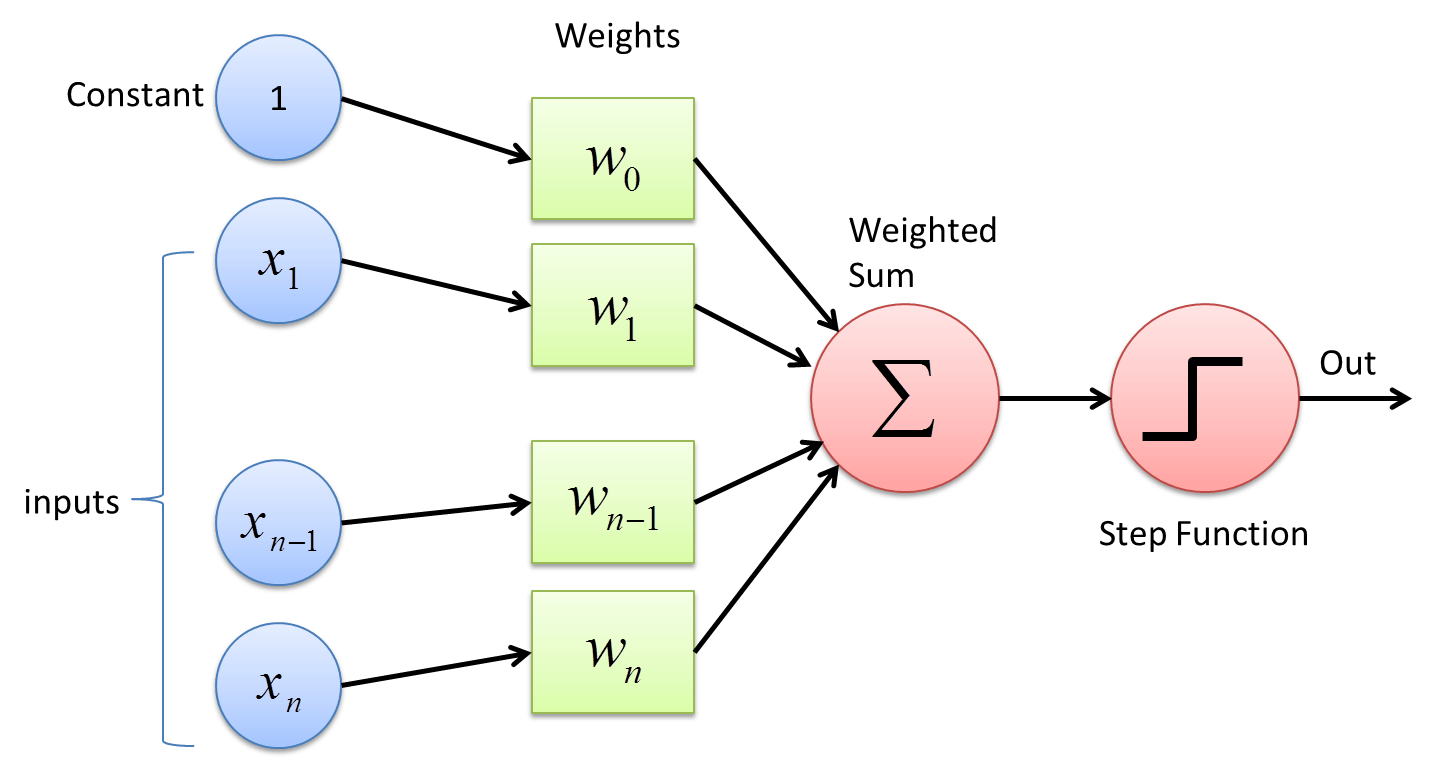
\includegraphics[width=0.50\textwidth]{media/perceptron.png}
        \caption{Perceptron model}
        \label{fig:perceptron}
    \end{figure}

    
    \subsection{Activation Function} \label{subsec:activation_funs}
    Τhe activation function defines the output of each node, given a set of inputs, that is, calculating the real value produced from \ref{eq:XY}.
    Multiple functions are used as activation functions in the development of NN's, such as the linear(identity), sign, sigmoid, hyperbolic tangent, ReLU, hard tanh and softmax functions. The fundamental activation function is the linear activation, which provides no non-linearity. Based on the type of classification combined with the number of classes, the most suitable activation is selected each time, so that the modeling power of the NN is the best possible for this task. The sign activation function, for example, can be used for binary classification. The sigmoid activation outputs a value y , where $y \subset (0,\ 1)$, which is preferable in cases of probabilistic computations(the prediction y' indicates the probability that the observed value, y, of the dependent variable is 1). The tanh function is usually used when the output of the computations is desired to be both positive and negative. Softmax results in probabilistic outputs, suitable for predicting one of multiple classes. ReLU is linear (identity function) for all positive values and zero for all negative values. The activation function is denoted by the symbol $\Phi$, so the prediction is calculated as follows: 
    \begin{equation} \label{eq:phi}
         y' = \Phi ( W · X  ) = \Phi ( \sum_{i=1}^{k} w\textsubscript{i} x\textsubscript{i} )
    \end{equation}
    where k is the number of input feature nodes. 
    Therefore, a neuron computes both functions of \ref{eq:phi} within the node.
   
    
    \subsection{Loss Function}
    Α loss(cost) function is a function that maps the value of one or more variables to a real number, representing the ``cost" of the event.
    The goal of the perceptron algorithm is to minimize the error in the prediction, therefore it is heuristically designed to minimise the number of misclassifications. The function that aims to minimise the value of the classification error(cost of classification), is called loss function. The choice of the loss function defines the outputs in a critical way and it is dependent on the application and the type of input data, as well as on the activation function used at that layer of the NN. In cases of numeric outputs, for example, a simple squared loss or hinge loss can be used. For a setting where the predictions are categorical, consider c the number of classes to be learned and y'\textsubscript{1},...,y'\textsubscript{c} the probabilities of the classes, with the rth class to be the ground-truth class, then for each instance, the loss function is calculated as follows: 
    \begin{equation}
        L = -\log(y'\textsubscript{r})
    \end{equation}
    This loss function is referred to as cross-entropy loss. 
    In detail, for each input data instance X or for a batch of them, the NN makes predictions used to calculate the error $E(X) = y - y'$, according to which the weights are updated. 
    The weight vector W is updated as follows:
    \begin{equation}
        W = W + a ( y - y' ) X
    \end{equation}
    The a factor controls the learning rate of the NN. What the perceptron algorithm does, is going over all the training data examples repeatedly in cycles and random order, while iteratively adjusting the weights until convergeance is achieved. Those cycles, are called epochs.
    
    \section{Feed - Forward Neural Networks}
    Multilayer NN's contain multiple hidden layers of computational units between the input and output layer. Those layers are referred to as hidden, because the computations performed are not visible to the user. Those successive layers, feed into one another in the forward direction from input to output. Those NN's, are known as feed-forward NN's. The number of nodes each layer has, is referred to as the dimensionality of this layer. In multi-layer networks, the loss is a complicated composition function of the weights in earlier layers.
    
    \begin{figure}[h]
        \centering
        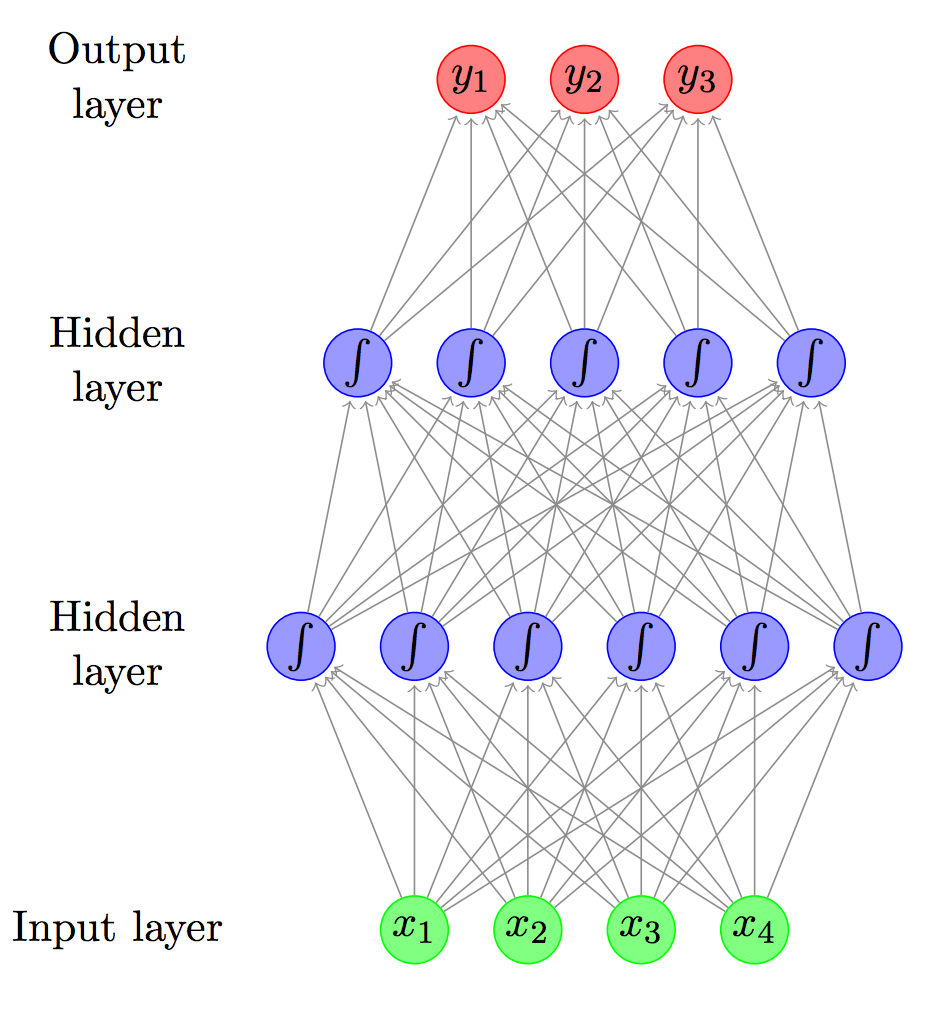
\includegraphics[width=0.50\textwidth]{media/Feed-forward-neural-network-with-two-hidden-layers.png}
        \caption{Feed-Forward NN structure}
        \label{fig:lstm}
    \end{figure}

    
    \subsection{Backpropagation}
    Multi-layer networks use various techniques in order to learn, the most popular of which is backpropagation. In this technique, the values produced by the NN as the output are compared with the correct answer, to calculate the value of the error function. The error is then fed back through the network, giving the information needed in order for the weights of each connection to be adjusted, so as to reduce the value of that error function as much as possible. After a large number of training cycles(epochs), the network will usually converge to a state where the computational error is small, which means that the NN was well trained and has learned a target function. 
    
    For the proper adjustment of the weights, a general method for non-linear optimization is used, referred to as the gradient descent. The network computes the derivative of the error function with respect to the network weights and changes the weights so that the error decreases (which means going downhill on the surface of the error function). That is the reason why backpropagation can only be applied on NN's with differentiable activation functions.

    The backpropagation algorithm contains two main phases, the forward and backward phase. During the forward phase the output and the loss are computed. Therefore, this phase initializes the intermediate variables that will be needed in the backward phase afterwards. The backward phase, uses the dynamic programming recurrence based on the multivariable chain rule of differential calculus. 
    More specifically, in the forward phase, the inputs for a training instance are fed into the NN, which results in a forward cascade of computations, where the values of each hidden layer are calculated, based on the current values of the weights across the layers. Those intermediate hidden and output variables will be required during the backward phase. After the completion of the computations, the prediction(final output) of the NN is calculated and compared to that of the training instance. Then, the derivative of the loss function with respect to the output is computed. The derivative of this loss afterwards, needs to be computed with respect to the weights in all layers in the backward phase.
    
    The main goal of the backward phase is to learn the gradient of the loss function with respect to the different weights by using the chain rule of differential calculus. These gradients are used to update the weights in all layers of the NN and are learned in the backward direction, starting from the output unit, where each node is processed exactly once in every pass. The learning process described above is known as the backward phase.
    
    \section{Recurrent Neural Networks (RNNs)} 
    
    \begin{figure}[h]
        \centering
        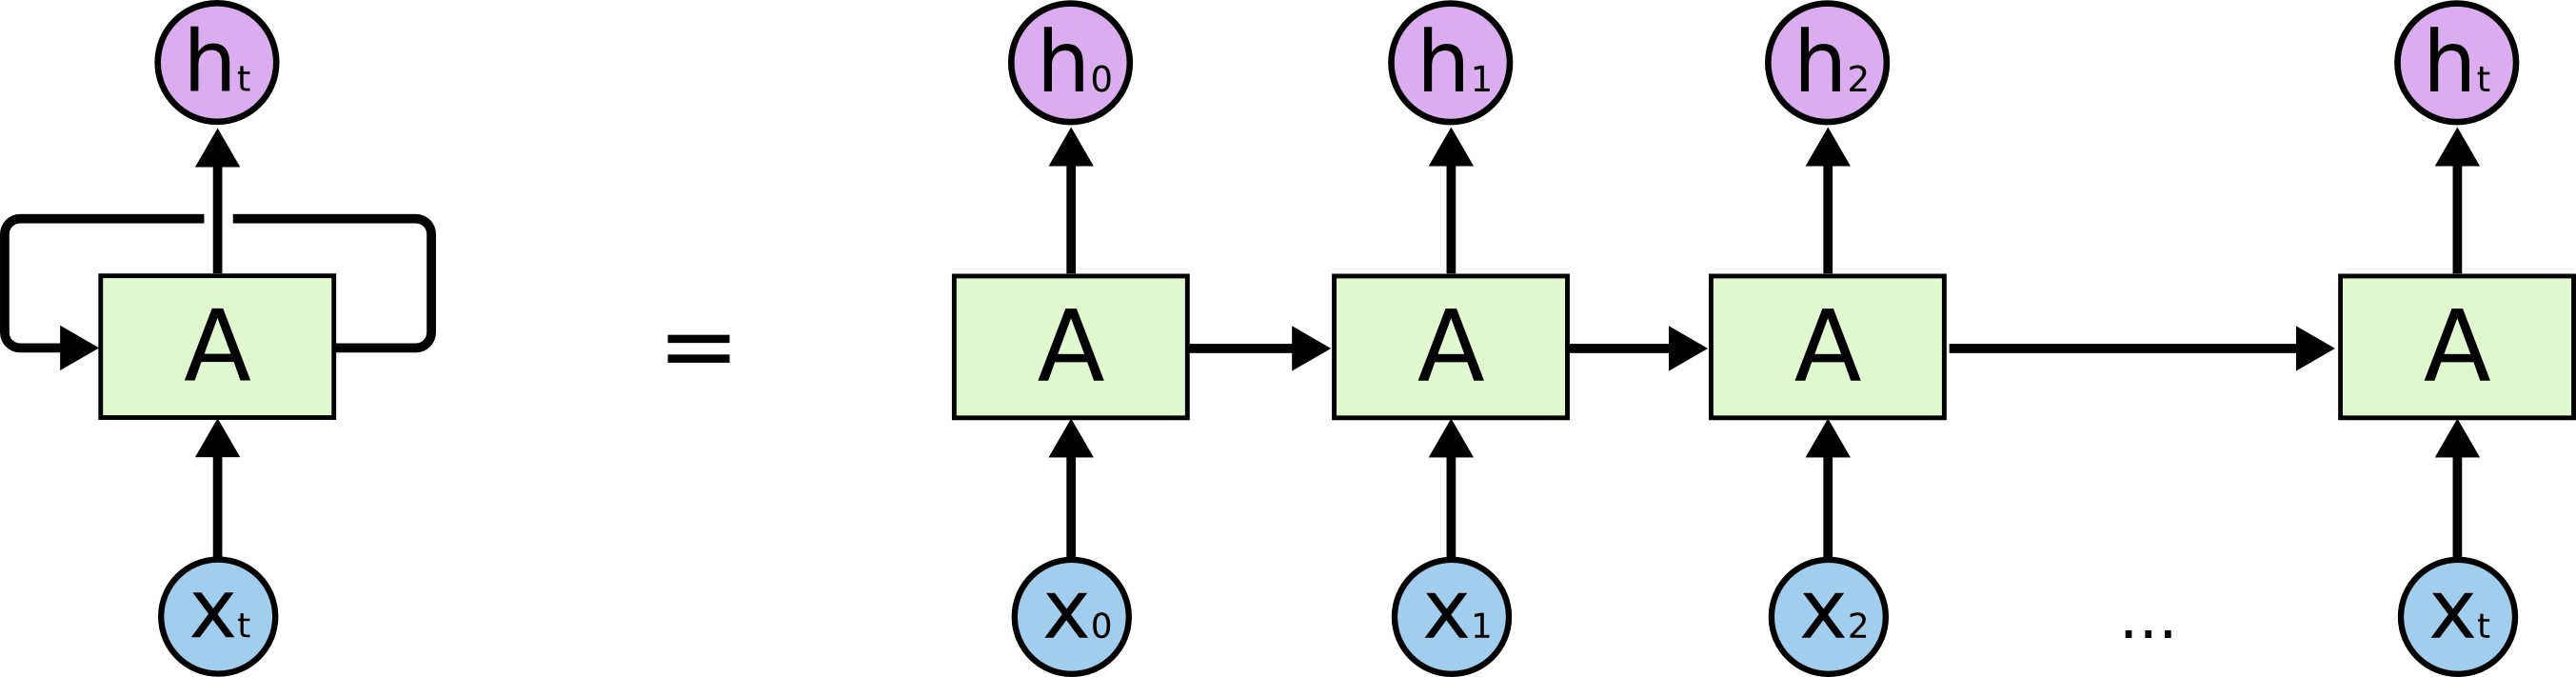
\includegraphics[width=0.65\textwidth]{media/RNN-unrolled.png}
        \caption{RNN unrolled}
        \label{fig:lstm}
    \end{figure}

    
    A recurrent neural network (RNN) is a feed-forward NN, where connections between nodes form a directed graph along a temporal sequence(series of items, e.g. a melody as a sequence of notes). This makes it capable of temporal dynamic behavior. This class of NNs can use their internal state (memory) to process sequences of inputs, unlike feed-forward NNs. The input of the RNN is an element x\textsubscript{t} of the sequence, where t represents the index or the time, and the expected output is next element x\textsubscript{t+1}. In other words, the RNN will be trained to predict the next element of a sequence. What makes the RNN capable to perform this task, is the action of reentering the hidden layer's output as an additional input. This way, the RNN can learn, not only based on the current item but also on its previous states, and thus, recursively, on the whole of the previous sequence. Therefore, an RNN can learn sequences, such as those of musical content. In such NNs, the input is of the form x\textsubscript{1} . . . x\textsubscript{n}, where x\textsubscript{t} is a d-dimensional point received at the time-stamp t. For instance, the vector x\textsubscript{t} might contain the d values at the t-th time-stamp of a multivariate time-series (with d different series). In a text-setting, the vector x\textsubscript{t} will contain the one-hot representation of the word at the t-th step . When a word is one-hot encoded, in a vector of length equal to the lexicon size, the component for this particular word has a value of 1 and all other components has a value of 0. The input x\textsubscript{t} of the RNN interacts with the hidden state produced from the inputs at previous time-steps, in a direct way. It is important that there is an input x\textsubscript{t} at each time-step, a hidden state h\textsubscript{t} that changes at each step as new data arrives and an output value y\textsubscript{t}. The hidden state at time-step t is given by a function of the input vector at step t and the hidden vector at step (t − 1): 
    \begin{equation}
        h\textsubscript{t} = f(h\textsubscript{t-1},x\textsubscript{t})
    \end{equation}
    The backpropagation algorithm in the case of RNNs, takes the temporal length into account when updating the weights during the learning process, which is a special type of algorithm, called backpropagation through time (BPTT).
    
    \subsection{ Long Short - Term Memory (LSTM)} \label{subsec:lstm}
    Training RNNs bears difficulties, due to the fact that they are deep time-layered networks, especially if the input sequence is very long. Thus, the depth of the temporal layering depends on the input data. However, even though the loss function has highly varying gradients to the variables in different layers, the parameter matrices are shared among different temporal layers, leading to unstable states. The main difficulties that emerge because of that, are the vanishing and exploding gradient during the update of the weights, specifically due to the successive multiplication of that shared weight matrix at backpropagation. A special class of RNNs, LSTMs, have been explicitly designed to deal with the vanishing gradient problem and they will be described below.
    LSTM is an RNN architecture which as such, has feedback connections and the ability to process not only single data points but also sequences of data, also capable of handling long-term dependencies. LSTMs have a chain like structure, where the repeating module consists of four NN layers, interacting in a very special way. The network's ability to model long-range dependencies and recognise patterns is achieved by using a gentle approach to update its cell states over time, so that there is greater persistence in the storage of certain information. Persistence in state values is exactly what eliminates the instability that occurs in the case of the vanishing and exploding gradient problems.

    \begin{figure}[h]
        \centering
        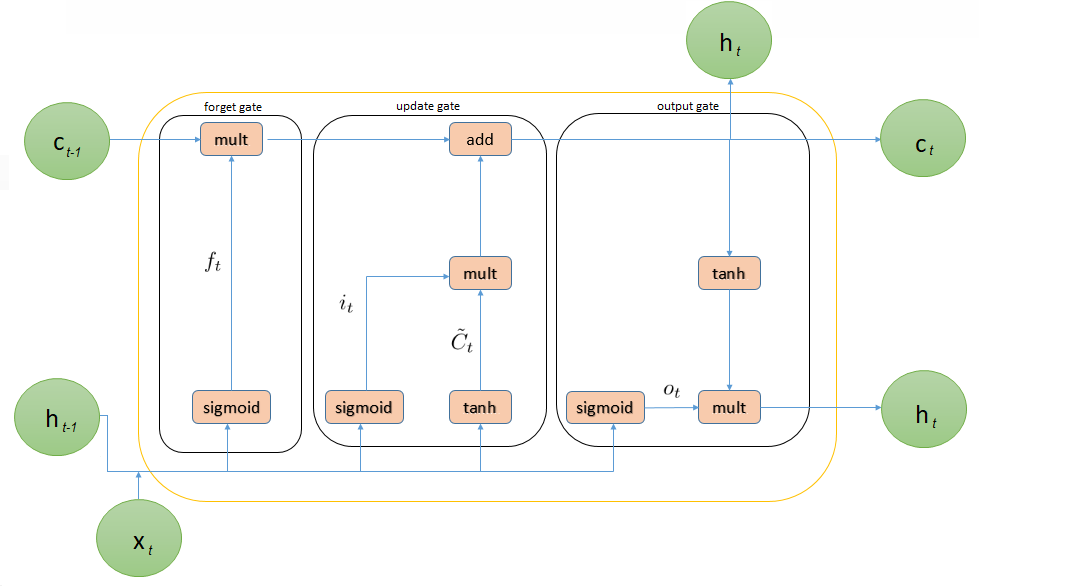
\includegraphics[width=0.65\textwidth]{media/lstm_simple.png}
        \caption{LSTM architecture}
        \label{fig:lstm}
    \end{figure}
    
    As we can see from figure \ref{fig:lstm}, there are three inputs (x\textsubscript{t}, h\textsubscript{t-1}, and c\textsubscript{t-1}) and two outputs (h\textsubscript{t} and c\textsubscript{t}) in the block, which are vectors carrying multiple values. Specifically, c\textsubscript{t-1} represents the input from a memory cell in time-stamp t, x\textsubscript{t} is a data input in step t, h\textsubscript{t} is the hidden state vector also known as output vector of the LSTM unit in time point t, that goes to both the output layer and the hidden layer in the next time-step. The key to LSTMs is the cell state, the line connecting input c\textsubscript{t-1} and output c\textsubscript{t} in figure \ref{fig:lstm} which runs straight down the entire chain of the NN, with only some minor linear interactions. It’s very easy for information to just flow along it unchanged. The LSTM has the ability to remove or add information to the cell state, controlled carefully by special structures, the gates. Gates optionally regulate the information that pass through. They consist of a sigmoid NN layer and a pointwise multiplication operation. The sigmoid layer produces numbers in range $( 0 \ 1 )$, a value that represents the percentage of each component to be let through. That is, based on the output of this sigmoid activation function, the valve will be completely closed, completely open or closed to some extent. A LSTM has three of these gates, to protect and control the cell state, which are called forget, update and output gates. For instance, when the forget valve(gate) in figure \ref{fig:lstm} above is open, memory flows from c\textsubscript{t-1} to c\textsubscript{t}. On the other hand, when the valve is closed, memory is cut off, and probably new memory will be added further in the pipeline.

    Specifically, the gates perform the following tasks:
    \begin{itemize}
        \item 
        The forget gate, manages what portion of the information from the previous state will be kept in the next state. It takes in the previous cell output h\textsubscript{t−1} and the current input band x\textsubscript{t}, applies the sigmoid activation layer so as to get values $\in (0,1)$, for each number in the cell state c\textsubscript{t−1} (equation \ref{eq:f}) and then performs element-wise multiplication with the old state from the previous unit.

        \item
        The update gate, updates the cell state based on the current input, by passing h\textsubscript{t−1} and x\textsubscript{t} into both a sigmoid activation layer (\ref{eq:i}) and tanh activation layer (\ref{eq:cellUpdate}), performing then an element-wise multiplication between the two results. The result from the previous operation is element-wisely added to the current state after applying the forget gate, to update the state with new information (equation \ref{eq:cellState}).    
       
        \item 
        Finally, the output gate controls what information gets passed on to the next state. A tanh activation layer is applied on the current state, to push the values in range $(-1,\ 1)$ and then an element-wise multiplication is performed, with the cell input (h\textsubscript{t−1} and x\textsubscript{t}) run through a sigmoid layer acting as a filter on what we decide to output. The output h\textsubscript{t} is then passed to the next layer of our network as one of the inputs.
        
    \end{itemize} 
    
    Therefore, summing up all of the above and as we can see from figure \ref{fig:lstm}, an LSTM unit takes x\textsubscript{t}, h\textsubscript{t-1}, and c\textsubscript{t-1} as inputs and after all the calculations and applications of its layers, it produces the h\textsubscript{t} and c\textsubscript{t} as outputs, which will be the inputs of the next LSTM unit, along with the data input of the next time-step  x\textsubscript{t+1}. The input x\textsubscript{t} is d-dimensional and the hidden states of the network are p-dimensional. The updates use four intermediate, p-dimensional vector variables $i,\ f,\ o$ and $C$. The intermediate variables $i,\ f$ and $o$ are respectively called input, forget, and output variables, because of the tasks they perform in the process of updating the cell and hidden states. Matrices $W \in \mathbb{R}\textsuperscript{$p\ x\ d$}$ and $U \in \mathbb{R}\textsuperscript{$p\ x\ p$}$ are the weight matrices and $b \in \mathbb{R}\textsuperscript{$p$} $ is the bias vector parameters, which all need to be learned during training, where $p$ is the number of hidden units and $d$ the number of features of the input data, as mentioned above.
    
    First, $f\textsubscript{t}$, $ i\textsubscript{t}$ and $ \Tilde{C}\textsubscript{t}$  are computed as follows:
    \begin{equation} \label{eq:f}
        f\textsubscript{t} = \sigma(\ W\textsubscript{f}\ x\textsubscript{t} + U\textsubscript{f}\ h\textsubscript{t-1} +  b\textsubscript{f}\ )
    \end{equation}
    
    \begin{equation} \label{eq:i}
        i\textsubscript{t} = \sigma(\ W\textsubscript{i}\ x\textsubscript{t} + U\textsubscript{i}\ h\textsubscript{t-1} +  b\textsubscript{i}\ )
    \end{equation}

    \begin{equation} \label{eq:cellUpdate}
        \Tilde{C}\textsubscript{t} = tanh(\ W\textsubscript{C}\ x\textsubscript{t} + U\textsubscript{C}\ h\textsubscript{t-1} +  b\textsubscript{C}\ )
    \end{equation}

    Then, the old cell state needs to be updated as well:
    
    \begin{equation} \label{eq:cellState}
        C\textsubscript{t} = f\textsubscript{t} * C\textsubscript{t-1} + i\textsubscript{t} * \Tilde{C}\textsubscript{t}
    \end{equation}

    Finally, the output will be computed, based on a filtered version of the updated cell state above, as follows:

     \begin{equation}
        o\textsubscript{t} = \sigma(\ W\textsubscript{o}\ x\textsubscript{t} + U\textsubscript{o}\ xh\textsubscript{t-1} +  b\textsubscript{o}\ )
    \end{equation}
    
    \begin{equation}
        h\textsubscript{t} = o\textsubscript{t} * tanh\ (C\textsubscript{t})
    \end{equation}
    
    
